\documentclass{article}
\usepackage[utf8]{inputenc}

\title{Übung 1}
\author{Laurenz Weixlbaumer, 11804751}
\date{Oktober 2018}

\renewcommand{\arraystretch}{1.5}
\renewcommand\thesubsection{(\alph{subsection})}

\usepackage{mathtools}

\begin{document}

\maketitle

\stepcounter{section}\stepcounter{section} % Start at 3
\section{Kombinatorische Schaltungen}
In dieser Aufgabe soll aufbauend aus einer textuellen Beschreibung eine Logikfunktion erstellt werden. Diese soll danach mittels Logikgattern realisiert und im letzten Schritt analysiert werden.

\subsection{Beschreibung als Schaltfunktion}

Die Funktion der Alarmanlage kann als
$$f_{alarm}(A,B,C,D) = (\overline{B} \land A) \lor (\overline{C} \land \overline{D}) \lor (\overline{A} \land \overline{D})$$
beschrieben werden, wobei $A..D$ die Eingänge A bis D repräsentieren.

\subsection{Kombinatorische Schaltung}

\begin{figure}[htp]
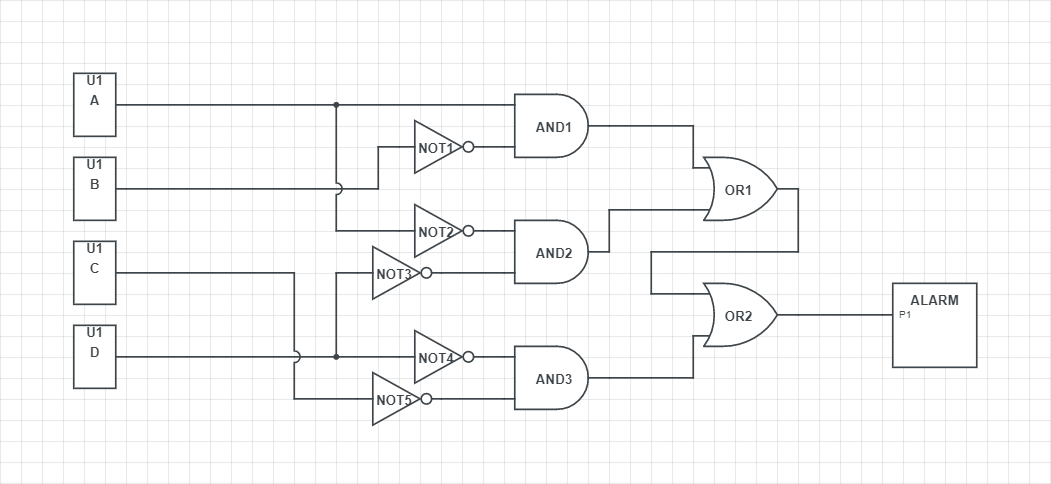
\includegraphics[width=\linewidth]{circuit.png}
\end{figure}

\subsection{Kosten der Schaltung}

In der Schaltung sind 10 Gatter zu finden, der längste Pfad durchläuft 5 Gatter.

\end{document}
